\documentclass[tikz, border=3.14mm]{standalone}
\usepackage{pgfplots}
\pgfplotsset{compat=1.18}
\usepgfplotslibrary{groupplots}

\begin{document}
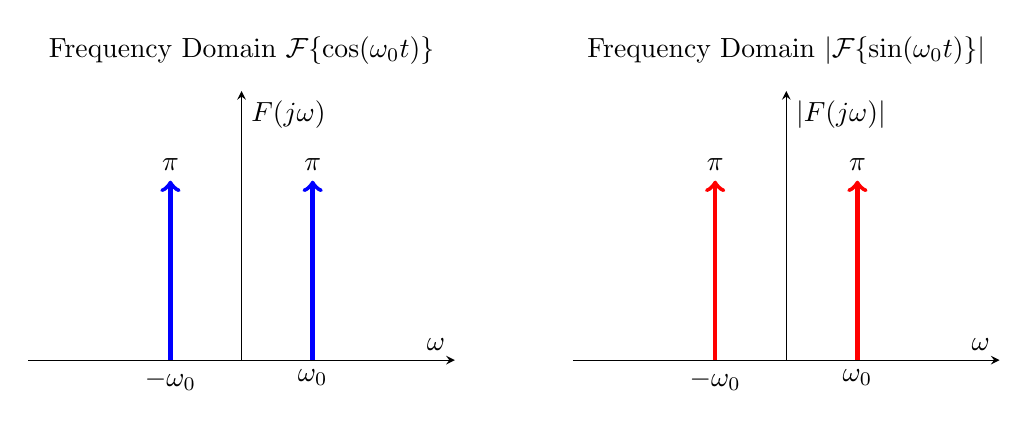
\begin{tikzpicture}
    \begin{groupplot}[
        group style={group size=2 by 1, horizontal sep=1.5cm},
        axis lines = middle,
        width = 7cm, height = 5cm,
        ymin = 0, ytick = \empty,
        xtick = \empty,
        grid=none
    ]
        % Cosine Spectrum
        \nextgroupplot[
            title = {Frequency Domain $\mathcal{F}\{\cos(\omega_0 t)\}$},
            xlabel = {$\omega$},
            ylabel = {$F(j\omega)$},
            xmin = -3, xmax = 3,
            ymax = 1.5,
            clip = false
        ]
        \draw[->, ultra thick, blue] (axis cs:1,0) -- (axis cs:1,1);
        \draw[->, ultra thick, blue] (axis cs:-1,0) -- (axis cs:-1,1);
        \node[anchor=north] at (axis cs:1, 0) {$\omega_0$};
        \node[anchor=north] at (axis cs:-1, 0) {$-\omega_0$};
        \node[anchor=south] at (axis cs:1, 1) {$\pi$};
        \node[anchor=south] at (axis cs:-1, 1) {$\pi$};

        % Sine Spectrum (Magnitude)
        \nextgroupplot[
            title = {Frequency Domain $|\mathcal{F}\{\sin(\omega_0 t)\}|$},
            xlabel = {$\omega$},
            ylabel = {$|F(j\omega)|$},
            xmin = -3, xmax = 3,
            ymax = 1.5,
            clip = false
        ]
        \draw[->, ultra thick, red] (axis cs:1,0) -- (axis cs:1,1);
        \draw[->, ultra thick, red] (axis cs:-1,0) -- (axis cs:-1,1);
        \node[anchor=north] at (axis cs:1, 0) {$\omega_0$};
        \node[anchor=north] at (axis cs:-1, 0) {$-\omega_0$};
        \node[anchor=south] at (axis cs:1, 1) {$\pi$};
        \node[anchor=south] at (axis cs:-1, 1) {$\pi$};

    \end{groupplot}
\end{tikzpicture}
\end{document}
